\documentclass[a4paper]{article}
\usepackage{geometry}
\usepackage{graphicx}
\usepackage{natbib}
\usepackage{amsmath}
\usepackage{amssymb}
\usepackage{amsthm}
\usepackage{paralist}
\usepackage{epstopdf}
\usepackage{tabularx}
\usepackage{longtable}
\usepackage{multirow}
\usepackage{multicol}
\usepackage[hidelinks]{hyperref}
\usepackage{fancyvrb}
\usepackage{algorithm}
\usepackage{algorithmic}
\usepackage{float}
\usepackage{paralist}
\usepackage[svgname]{xcolor}
\usepackage{enumerate}
\usepackage{array}
\usepackage{times}
\usepackage{url}
\usepackage{fancyhdr}
\usepackage{comment}
\usepackage{environ}
\usepackage{times}
\usepackage{textcomp}
\usepackage{caption}
\usepackage{color}
\usepackage{xcolor}

\urlstyle{rm}

\setlength\parindent{0pt} % Removes all indentation from paragraphs
\theoremstyle{definition}
\newtheorem{definition}{Definition}[]
\newtheorem{conjecture}{Conjecture}[]
\newtheorem{example}{Example}[]
\newtheorem{theorem}{Theorem}[]
\newtheorem{lemma}{Lemma}
\newtheorem{proposition}{Proposition}
\newtheorem{corollary}{Corollary}

\floatname{algorithm}{Procedure}
\renewcommand{\algorithmicrequire}{\textbf{Input:}}
\renewcommand{\algorithmicensure}{\textbf{Output:}}
\newcommand{\abs}[1]{\lvert#1\rvert}
\newcommand{\norm}[1]{\lVert#1\rVert}
\newcommand{\RR}{\mathbb{R}}
\newcommand{\CC}{\mathbb{C}}
\newcommand{\Nat}{\mathbb{N}}
\newcommand{\br}[1]{\{#1\}}
\DeclareMathOperator*{\argmin}{arg\,min}
\DeclareMathOperator*{\argmax}{arg\,max}
\renewcommand{\qedsymbol}{$\blacksquare$}

\definecolor{dkgreen}{rgb}{0,0.6,0}
\definecolor{gray}{rgb}{0.5,0.5,0.5}
\definecolor{mauve}{rgb}{0.58,0,0.82}

\newcommand{\Var}{\mathrm{Var}}
\newcommand{\Cov}{\mathrm{Cov}}

\newcommand{\vc}[1]{\boldsymbol{#1}}
\newcommand{\xv}{\vc{x}}
\newcommand{\Sigmav}{\vc{\Sigma}}
\newcommand{\alphav}{\vc{\alpha}}
\newcommand{\muv}{\vc{\mu}}

\newcommand{\red}[1]{\textcolor{red}{#1}}

\def\x{\mathbf x}
\def\y{\mathbf y}
\def\w{\mathbf w}
\def\v{\mathbf v}
\def\E{\mathbb E}
\def\V{\mathbb V}

% TO SHOW SOLUTIONS, include following (else comment out):
\newenvironment{soln}{
    \leavevmode\color{blue}\ignorespaces
}{}


\hypersetup{
%    colorlinks,
    linkcolor={red!50!black},
    citecolor={blue!50!black},
    urlcolor={blue!80!black}
}

\geometry{
  top=1in,            % <-- you want to adjust this
  inner=1in,
  outer=1in,
  bottom=1in,
  headheight=3em,       % <-- and this
  headsep=2em,          % <-- and this
  footskip=3em,
}


\pagestyle{fancyplain}
\lhead{\fancyplain{}{Homework 2}}
\rhead{\fancyplain{}{CS 760 Machine Learning}}
\cfoot{\thepage}

\title{\textsc{Homework 2}} % Title

%%% NOTE:  Replace 'NAME HERE' etc., and delete any "\red{}" wrappers (so it won't show up as red)

\author{
\red{$>>$Martin Diges$<<$} \\
\red{$>>$9080689699$<<$}\\
} 

\date{}

\begin{document}

\maketitle 


\textbf{Instructions:} 
Use this latex file as a template to develop your homework. Submit your homework on time as a single pdf file to Canvas. Please wrap your code and upload to a public GitHub repo, then attach the link below the instructions so that we can access it. You can choose any programming language (i.e. python, R, or MATLAB), as long as you implement the algorithm from scratch (e.g. do not use sklearn on questions 1 to 7 in section 2). Please check Piazza for updates about the homework.
\\\\
\hypersetup{colorlinks=true, linkcolor=cyan}
\url{https://github.com/missingnoglitch0/760_hw2}

\red{PLEASE SEE THE README.md IN THE REPOSITORY FOR INFO HELPFUL FOR GRADING}

\section{A Simplified Decision Tree}
You are to implement a decision-tree learner for classification.
To simplify your work, this will not be a general purpose decision tree.  Instead, your program can assume that
\begin{itemize}
\item each item has two continuous features $\x \in \RR^2$
\item the class label is binary and encoded as $y \in \{0,1\}$
\item data files are in plaintext with one labeled item per line, separated by whitespace:
$$x_{11} \quad x_{12} \quad y_1$$
$$...$$
$$x_{n1} \quad x_{n2} \quad y_n$$
\end{itemize}

Your program should implement a decision tree learner according to the following guidelines:
\begin{itemize}
\item Candidate splits $(j,c)$ for numeric features should use a threshold $c$ in feature dimension $j$ in the form of $x_{j}\ge c$.
\item $c$ should be on values of that dimension present in the training data; i.e. the threshold is on training points, not in between training points. You may enumerate all features, and for each feature, use all possible values for that dimension.
\item You may skip those candidate splits with zero split information (i.e. the entropy of the split), and continue the enumeration.
\item The left branch of such a split is the ``then'' branch, and the right branch is ``else''.
\item Splits should be chosen using information gain ratio. If there is a tie you may break it arbitrarily.
\item The stopping criteria (for making a node into a leaf) are that 
	\begin{itemize}
	\item the node is empty, or
	\item all splits have zero gain ratio (if the entropy of the split is non-zero), or
	\item the entropy of any candidates split is zero
	\end{itemize}
\item To simplify, whenever there is no majority class in a leaf, let it predict $y=1$.
\end{itemize}

\section{Questions}
\begin{enumerate}
\item (Our algorithm stops at pure labels) [10 pts] If a node is not empty but contains training items with the same label, why is it guaranteed to become a leaf?  Explain. You may assume that the feature values of these items are not all the same. \\

Supposing the label shared by all items is $q$, we know that for any $i \neq q$, $P(i) = 0$ and $P(q) = 1$. Thus, the entropy of these items will be $\sum_{i=1}^{k} P(i) \log_{2}{P(i)} = 0 + ... + 1 * \log_{2}{1} + ... + 0 = 1(0) = 0$. 
One of our stopping conditions is that the entropy of any candidate splits is zero, which is the case here. Note that this is the case because $H_D(Y) = 0 \longleftrightarrow H_D(S) = 0$ for any split $S$. Intuitively, there is no further information that can be gained from this point on.

\item (Our algorithm is greedy)  [10 pts] Handcraft a small training set where both classes are present but the algorithm refuses to split; instead it makes the root a leaf and stop;
Importantly, if we were to manually force a split, the algorithm will happily continue splitting the data set further and produce a deeper tree with zero training error.
You should (1) plot your training set, (2) explain why.  Hint: you don't need more than a handful of items. \\

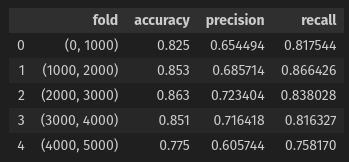
\includegraphics[]{hw2/2_2.png}

This training set consists of the points $(1,1,1)$, $(1,2,0)$, $(2,2,1)$, $(2,1,0)$
We note that our heuristic of using a gain ratio will result in gain ratios of 0 regardless of the initial split. 

Without loss of generality, if we spit by the first (or second) feature between its values 1 and 2, we notice that both the original points and split children both have $P(Y=1) = P(Y=0) = 0.5$. Additionally, splits result in children with equal numbers of data points.
Thus, \\$H_D(Y) = -(0.5 \log_{2}{0.5} + 0.5 \log_{2}{0.5}) = -(0.5*-1 + 0.5*-1) = -(-1) = 1$ and\\
$H_D(Y) = H_D(child) \implies H_D(Y | S) = 0.5 * H_D(child) + 0.5 * H_D(child) = H_D(child) = 1$
\\Finally, we have that $InfoGain = H_D(Y) - H_D(Y | S) = 1 - 1 = 0$.
Splits by either feature will have InfoGain=0, meaning GainRatio=0, meaning our algorithm will not split.

Should we manually force a split on a feature $X_j$, however, we note that each child will have variation in both $X_{not j}$ and $Y$. Thus, our algorithm will proceed and split both children.

\item (Information gain ratio exercise)  [10 pts] Use the training set Druns.txt.  For the root node, list all candidate cuts and their information gain ratio. If the entropy of the candidate split is zero, please list its mutual information (i.e. information gain). Hint: to get $\log_2(x)$ when your programming language may be using a different base, use \verb|log(x)/log(2)|. Also, please follow the split rule in the first section. \\

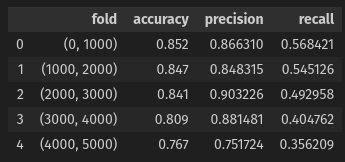
\includegraphics[width=0.8\textwidth]{hw2/2_3.png}

\item (The king of interpretability)  [10 pts] Decision tree is not the most accurate classifier in general.  However, it persists.  This is largely due to its rumored interpretability: a data scientist can easily explain a tree to a non-data scientist.  Build a tree from D3leaves.txt.  Then manually convert your tree to a set of logic rules.  Show the tree\footnote{When we say show the tree, we mean either the standard computer science tree view, or some crude plaintext representation of the tree -- as long as you explain the format.  When we say visualize the tree, we mean a plot in the 2D $\x$ space that shows how the tree will classify any points.} and the rules. \\

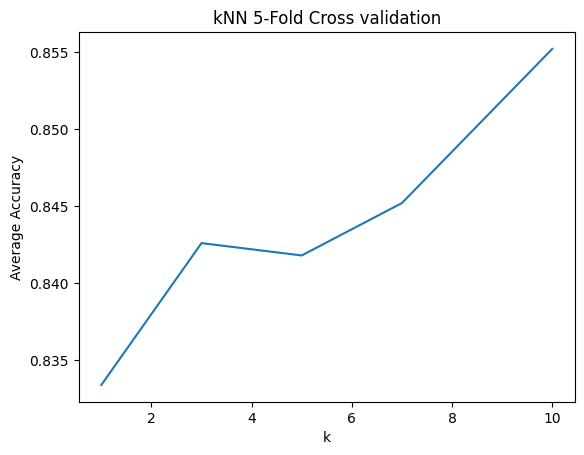
\includegraphics[width=0.4\textwidth]{hw2/2_4.png}\\
Our tree is rooted at the top leftmost node. A node can appear as one of two strings:
\begin{enumerate}
    \item $X[j] \geq c$, where $j$ is the index of a feature in $X$ and $c$ is a threshold. This node asks whether the $j$-th feature of a data point meets the threshold $c$. If it does, proceed to the $l$ node shown below $c$. If not, proceed to $r$.
    \item $0$ or $1$. This node's string indicates the prediction at which the tree has arrived.
\end{enumerate}

\item (Or is it?)  [10 pts] For this question only, make sure you DO NOT VISUALIZE the data sets or plot your tree's decision boundary in the 2D $\x$ space.  If your code does that, turn it off before proceeding.  This is because you want to see your own reaction when trying to interpret a tree.  You will get points no matter what your interpretation is.
And we will ask you to visualize them in the next question anyway.
  \begin{itemize}
  
  \item Build a decision tree on D1.txt.  Show it to us in any format (e.g. could be a standard binary tree with nodes and arrows, and denote the rule at each leaf node; or as simple as plaintext output where each line represents a node with appropriate line number pointers to child nodes; whatever is convenient for you). Again, do not visualize the data set or the tree in the $\x$ input space.  In real tasks you will not be able to visualize the whole high dimensional input space anyway, so we don't want you to ``cheat'' here. 

  \includegraphics[width=0.4\textwidth]{hw2/2_5_1.png}\\
  
  \item Look at your tree in the above format (remember, you should not visualize the 2D dataset or your tree's decision boundary) and try to interpret the decision boundary in human understandable English. 

    This decision tree, when you simplify the conditional logic, says that if $X[1] >= 0.36$ OR $X[0] >= 0.25$, the classification label will be 1. Otherwise, the classification label will be 0.
    In plain english, if at least one of the features of a data point excedes a feature-specific threshold, we will obtain a 1, otherwise a 0.
  
  \item Build a decision tree on D2.txt.  Show it to us. 

    \includegraphics[width=0.4\textwidth]{hw2/2_5_2.png}\\
  
  \item Try to interpret your D2 decision tree. Is it easy or possible to do so without visualization? \\

    My interpretation of this tree is that, for a data point to receive a class label of 1, it must meet a threshold for its feature 1. If its feature 0 meets a threshold (0.53), then threshold feature 1 must meet will be lesser (0.42) than in the remaining case (0.53).
    On a 2D plane, I interpret this tree as two pass-fail regions which are parallel to the axis of feature 0 but are discontinuous, their border with each other being at 0.53 X[0].
    As the number of features or values they can take on grows, this could get really messy.
  
  \end{itemize}

\item (Hypothesis space)  [10 pts] For D1.txt and D2.txt, do the following separately:
  \begin{itemize}
  
  \item Produce a scatter plot of the data set.

  \item Visualize your decision tree's decision boundary (or decision region, or some other ways to clearly visualize how your decision tree will make decisions in the feature space).

  For D1.txt\\
  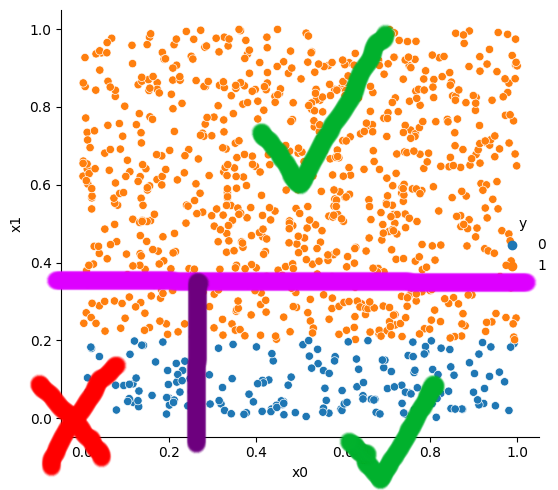
\includegraphics[width=0.4\textwidth]{hw2/2_6_1_boundary.png}\\

  For D2.txt\\
  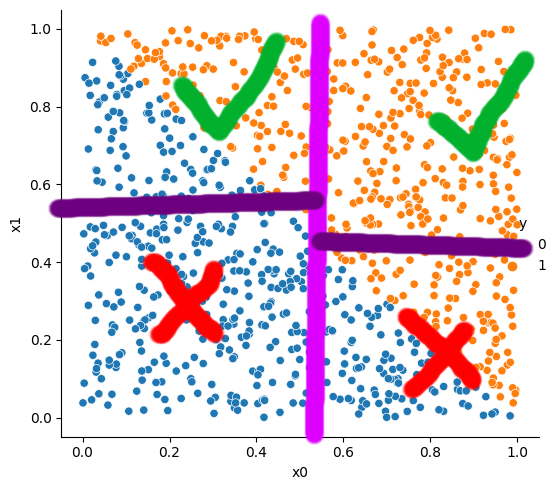
\includegraphics[width=0.4\textwidth]{hw2/2_6_2_boundary.png}\\

  \end{itemize}
Then discuss why the size of your decision trees on D1 and D2 differ.  Relate this to the hypothesis space of our decision tree algorithm. \\

    The hypothesis space of our decision tree algorithm seems to be binary functions with respect to input features.

    Our algorithm will attempt to split a region whenever data are not well predicted by the side of a boundary that region is on.

    The decision tree algorithm will not be able to predict well for functions such as those seen in D2, e.g. summation of features, because they are not within its hypothesis space and thus will split again on both sides of the decision boundary.

\item (Learning curve)  [20 pts] We provide a data set Dbig.txt with 10000 labeled items.  Caution: Dbig.txt is sorted.
  \begin{itemize}
  
  \item You will randomly split Dbig.txt into a candidate training set of 8192 items and a test set (the rest).  Do this by generating a random permutation, and split at 8192.
  
  \item Generate a sequence of five nested training sets $D_{32} \subset D_{128} \subset D_{512} \subset D_{2048} \subset D_{8192}$ from the candidate training set.  The subscript $n$ in $D_n$ denotes training set size.  The easiest way is to take the first $n$ items from the (same) permutation above.  This sequence simulates the real world situation where you obtain more and more training data.
  
  \item For each $D_n$ above, train a decision tree.  Measure its test set error $err_n$.  Show three things in your answer: (1) List $n$, number of nodes in that tree, $err_n$. (2) Plot $n$ vs. $err_n$.  This is known as a learning curve (a single plot). (3) Visualize your decision trees' decision boundary (five plots). \\

    1.
    \begin{itemize}
        \item $D_{32}$ (32, 5, 0.27876106194690264)
        \item $D_{128}$ (128, 5, 0.25719026548672563)
        \item $D_{512}$ (512, 7, 0.23949115044247793)
        \item $D_{2048}$ (2048, 7, 0.2372787610619469)
        \item $D_{8192}$ (8192, 7, 0.23672566371681414)
    \end{itemize}

    2.
    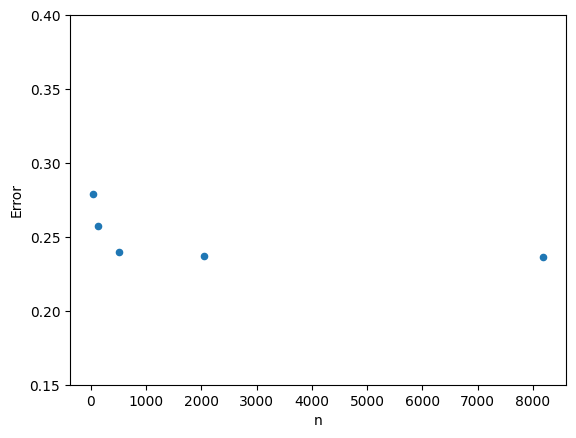
\includegraphics[width=0.8\textwidth]{hw2/2_7_2.png}\\

    3.
    \begin{itemize}
        \item $D_{32}$ 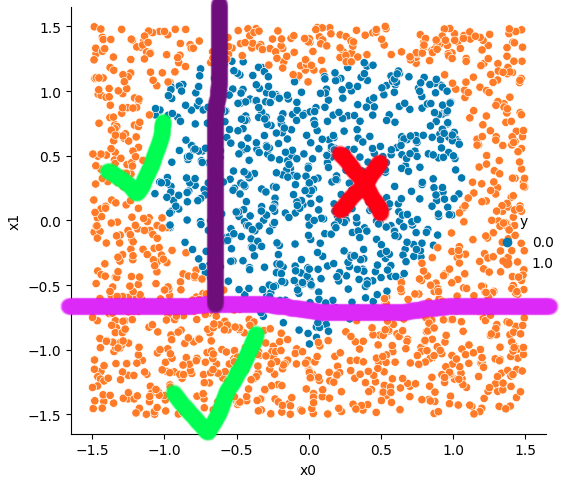
\includegraphics[width=0.8\textwidth]{hw2/2_7_3_1.png}\\
        \item $D_{128}$ 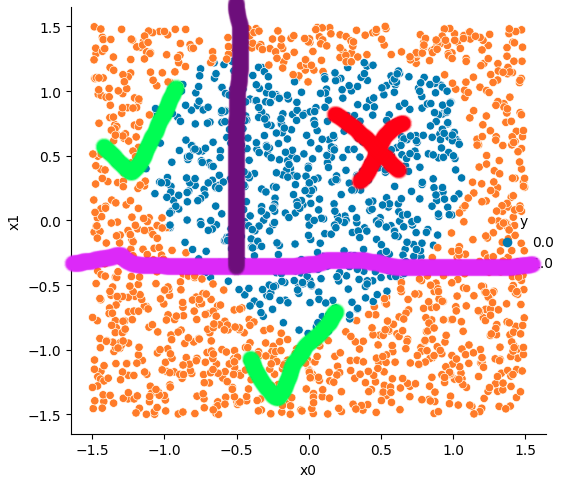
\includegraphics[width=0.8\textwidth]{hw2/2_7_3_2.png}\\
        \item $D_{512}$ 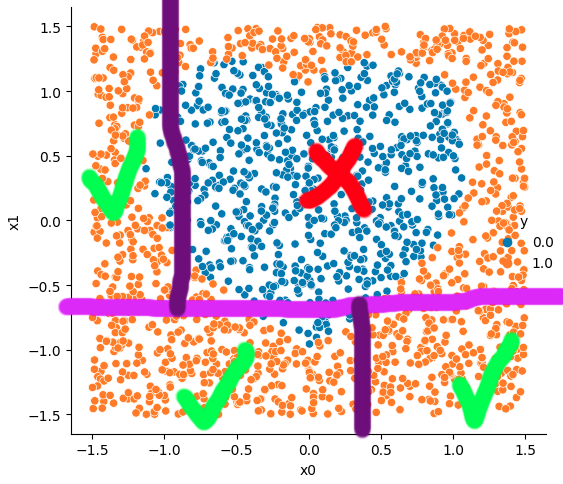
\includegraphics[width=0.8\textwidth]{hw2/2_7_3_3.png}\\
        \item $D_{2048}$ 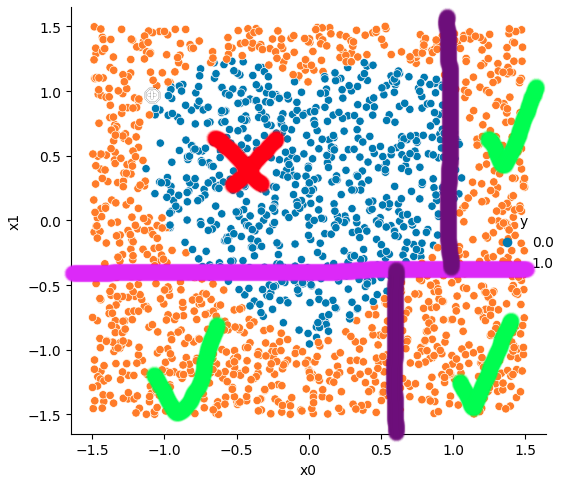
\includegraphics[width=0.8\textwidth]{hw2/2_7_3_4.png}\\
        \item $D_{8192}$ 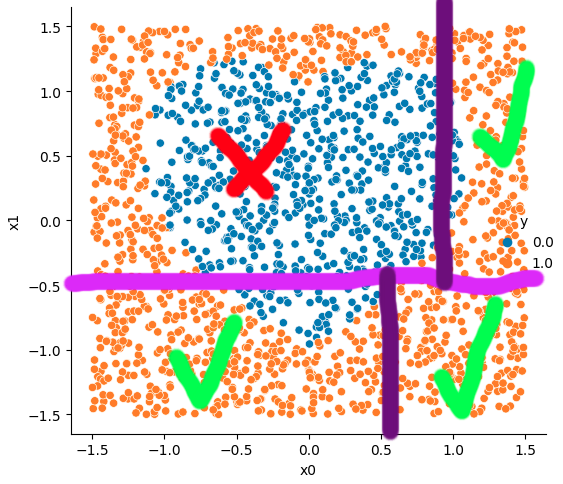
\includegraphics[width=0.8\textwidth]{hw2/2_7_3_5.png}\\
    \end{itemize}
  
  \end{itemize}
  
\end{enumerate}

\section{sklearn [10 pts]}
Learn to use sklearn (\url{https://scikit-learn.org/stable/}).
Use sklearn.tree.DecisionTreeClassifier to produce trees for datasets $D_{32}, D_{128}, D_{512}, D_{2048}, D_{8192}$.  Show two things in your answer: (1) List $n$, number of nodes in that tree, $err_n$. (2) Plot $n$ vs. $err_n$.

1.
\begin{itemize}
        \item $D_{32}$ (32, 4+3, 0.28871681415929207)
        \item $D_{128}$ (128, 3+2, 0.2936946902654868)
        \item $D_{512}$ (512, 4+3, 0.30918141592920356)
        \item $D_{2048}$ (2048, 4+3, 0.2981194690265486)
        \item $D_{8192}$ (8192, 4+3, 0.31969026548672563)
    \end{itemize}
    Note that scikit's tree does not have a way to return the number of nodes, only leaves, but we can deduce the number of inner nodes by knowing that each node either splits into two (internal) or has no children (leaf). 4 leaves implies 3 internal nodes, 3 leaves implies 2 internal nodes, with 1 leaf coming directly off the root node.

2.
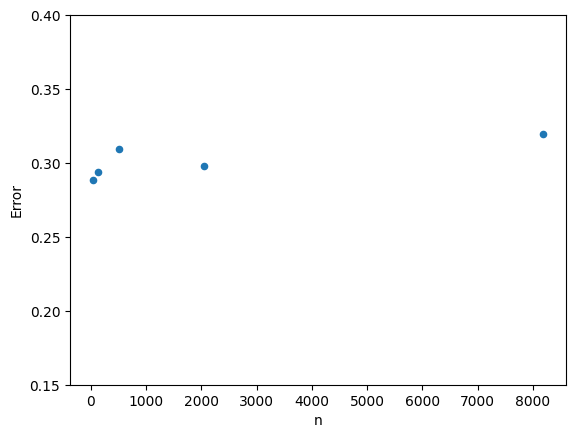
\includegraphics[width=0.8\textwidth]{hw2/3_2.png}\\

\newpage
\section{Lagrange Interpolation [10 pts]}
Fix some interval $[a, b]$ and sample $n = 100$ points $x$ from this interval uniformly. Use these to build a training set consisting of $n$ pairs $(x, y)$ by setting function $y = sin(x)$. \\

Build a model $f$ by using Lagrange interpolation, check more details in \url{https://en.wikipedia.org/wiki/Lagrange_polynomial} and \url{https://docs.scipy.org/doc/scipy/reference/generated/scipy.interpolate.lagrange.html}. \\

Generate a test set using the same distribution as your test set. Compute and report the resulting model’s train and test error. What do you observe?
Repeat the experiment with zero-mean Gaussian noise $\epsilon$ added to $x$. Vary the standard deviation for $\epsilon$ and report your findings.
\\
\\
I observe that as we increase $\epsilon$, the model's test error seems to decrease.
\\
\\
\\For std dev = 0 (i.e. the base input dataset before adding noise):
\\- train log mean squared error = 334.43622749096517
\\- test log mean squared error = 334.6563799257306
\\For std dev = 0.01:
\\- train log mean squared error = 333.8524226649329
\\- test log mean squared error = 333.8384908119607
\\For std dev = 0.1:
\\- train log mean squared error = 344.03565365413317
\\- test log mean squared error = 344.9000597801279
\\For std dev = 1:
\\- train log mean squared error = 356.82613749985626
\\- test log mean squared error = 315.22368624964537
\\For std dev = 10:
\\- train log mean squared error = 287.27468349526106
\\- test log mean squared error = 70.66524084120545
\\For std dev = 100:
\\- train log mean squared error = 262.1043764431617
\\- test log mean squared error = -13.074606868655378

\bibliographystyle{apalike}
\end{document}
